%%%%%%%%%%%%%%%%%%%%%%%%%%%%%%%%%%%%%
% Note: This document can be build  %
% by using pdflatex and not latex   %
%%%%%%%%%%%%%%%%%%%%%%%%%%%%%%%%%%%%%
%
% Lade Dokumenttyp
% Die Kommentare zu diesem Befehl sind etwas länglich und stehen in latex/documentclass.tex
% Das sollte man sich mal durchlesen!
\documentclass[a4paper, 12pt, BCOR8.25mm, headsepline, final, bibliography=totoc, listof=totoc, index=totoc, parskip=half*, chapterprefix, appendixprefix, captions=nooneline, origlongtable]{scrbook}
%
% Lade Unterstützung für die deutsche Sprache
%
%%%%%%%%%%%%%%%%%%%
% Sprachcodierung %
%%%%%%%%%%%%%%%%%%%
\usepackage[T1]{fontenc}
% Paket fontenc: Fontencoding T1 festlegen, damit Wörter, die Umlaute
% enthalten richtig getrennt werden.
\usepackage[utf8]{inputenc}
% Paket inputenc: Unterstützung verschiedener Zeichenkodierungen.  Unterstützte
% Kodierungen sind:
% ascii		ASCII Kodierung für Zeichen in dem Bereich von 32 bis 127
% latin1	ISO Latin1
% latin2	ISO Latin2
% latin3	ISO Latin3
% latin4	ISO Latin4
% latin5	ISO Latin5
% latin9	ISO Latin9 (definiert die ISO 8859-15 Codierung einschließlich des EURO-Zeichnes: \texteuro)
% decmulti	DEC Multinational Character Set Encoding für das OpenVMS Betriebssystem
% cp437		IBM 437 Code Page
% cp437de	IBM 437 Code Page deutsche Version
% cp850		IBM 850 Code Page
% cp852		IBM 852 Code Page
% cp865		IBM 850 Code Page
% cp1250	Windows 1250 (Zentral- und Osteuropa) Code Page
% cp1252	Synonym für ansinew
% applemac	Macintosh Kodierung
% next		Next Kodierung
% ansinew	Windows 3.1 ANSI Kodierung, erweiterung von Latin1
% Dokumentation zu diesem Paket: /usr/share/doc/texmf/latex/base/inputenc.dvi.ps
%
\usepackage[english,ngerman]{babel}
% Paket babel: Unterstützung für andere Sprachen als amerikanisches Englisch
% Die Sprachen Englisch, Französich und Deutsch  verwenden. Die zuletzt aufgeführte
% Sprache ist die Sprache, die beim Start geladen wird. Zwischen den einzelnen
% Sprachen kann man mittels \selectlanguage{english}, \selectlanguage{ngerman} und
% \selectlanguage{french} umgeschaltet werden. ngerman steht für die neue, german
% für die alte deutsche Rechtschreibung.
% Mittels \iflanguage{sprache}{wahr-Klausel}{falsch-Klausel} kann abgeprüft werden,
% welche Sprache gerade aktiv ist und demensprechend können Befehle ausgeführt werden.
% Umlaute und Sonderzeichen mit dem babel Paket:
% ä = \"a 
% Ä = \"A
% ö = \"o 
% Ö = \"O
% ü = \"u 
% Ü = \"U
% ß = \"s
% SS = \"S ( groß geschriebene ß als SS wie z.B in STRASSE )
% Deutsche doppelte Anführungszeichen links unten \glqq
% Deutsche doppelte Anführungszeichen rechts oben \grqq
% Deutsche einfache Anführungszeichen links unten \glq
% Deutsche einfache Anführungszeichen rechts      \grq
% Französische doppelte Anführungszeichen links  \flqq
% Französische doppelte Anführungszeichen rechts \frqq
% Franz<F6>sische einfache Anf<FC>hrungszeichen links  \flq
% Franz<F6>sische einfache Anf<FC>hrungszeichen rechts \frq
% Original Anf<FC>hrungszeichen \dq
% Weitere Spezialbefehle zur Silbentrennung und Lignatur
% Dokumentation zu diesem Paket: /usr/share/doc/texmf/generic/babel/user.dvi.gz
\selectlanguage{ngerman}

%
% Lade persönliche Daten
% Dieses Dokument solltest Du auf jeden Fall anpassen, denn hier kommt Dein Name und der Titel Deiner Arbeit hinein.
% Hier werden Makros definiert, die in den folgenden LaTeX-Dokumenten verwendet werden.
%
%
% Die Art der Arbeit: Bachelorarbeit/Masterarbeit - einfach das richtige auskommentieren
% 
%\newcommand{\thethesis}[0]{Masterarbeit}
\newcommand{\thethesis}[0]{Masterprojekt}
%
% Der Titel Deiner Arbeit
%
\newcommand{\thesistitle}[0]{Ausarbeitung zum Projekt QPI-SQL}
%
% Der formatierte Titel Deiner Arbeit für das erste Deckblatt
%
\newcommand{\thesisTitleFormatted}[0]{Ausarbeitung zum Projekt QPI-SQL}
%
% Das Thema Deiner Arbeit (Kurzfassung des Titels)
%
\newcommand{\thesissubject}[0]{\thesistitle}
%
% Stichwörter, die Deine Arbeit charakterisieren
%
\newcommand{\thesiskeywords}[0]{Ilias; Masterprojekt; Plugin; SQL; StudOn; FAU; INF6; Datenmanagement; Dominik; Probst}
%
% Beginn Deiner Arbeit
%
\newcommand{\startofwork}[0]{01.10.2018}
%
% Abgabetag Deiner Arbeit
%
\newcommand{\dayofdoom}[0]{30.05.2019}
%
% Der Betreuer Deiner Arbeit
%
\newcommand{\tutor}{M. Sc. Andreas Maximilian Wahl}
%
% Dein Korrektor bzw. Professor
%
\newcommand{\corrector}[0]{Prof. Dr. Richard Lenz}
%
% Dein Vor- und Nachname
%
\newcommand{\myname}[0]{Dominik Probst}
%
% Dein Geburtstag
%
\newcommand{\birthday}[0]{23.06.1995}
%
% Dein Geburtsort
%
\newcommand{\birthplace}[0]{Nürnberg}

%
% Lade Pakete
%
%%%%%%%%%%%%
% Tabellen %
%%%%%%%%%%%%
% Paket supertabular: Aufteilung von Tabellen auf mehrere Seiten bzw.
% Einbindung mehrseitige Tabellen. Die sind dann auch wirklich da, wo man sie vom Layout her hinsetzt :-)
\usepackage{multicol}
\usepackage{supertabular}
%
% Paket colortbl: Farbige Tabellenspalten
% Documentation:  CTAN:macros/latex/contrib/colortbl
\usepackage{colortbl}
%
% Paket booktabs: Trennlinien für Tabellen
\usepackage{booktabs}
%
%%%%%%%%%%%%%%%%%%%%%%%%%
% Programmcode Listings %
%%%%%%%%%%%%%%%%%%%%%%%%%
\usepackage{listings}
%
%%%%%%%%%
% Index %
%%%%%%%%%
% Paket makeidx: Zur Erstellung eines Index
\usepackage{makeidx}
% Erstellt einen Index
\makeindex
%
%%%%%%%%%%%%%%%%%%%%%%%%%%%%%%
% Bessere Bildunterschrfiten %
%%%%%%%%%%%%%%%%%%%%%%%%%%%%%%
\usepackage[justification=centerlast,format=hang,font=small,labelfont=bf]{caption}
%
%%%%%%%%%
% Farbe %
%%%%%%%%%
\usepackage{color}
%
%%%%%%%%%%%%
% Grafiken %
%%%%%%%%%%%%
% PDF als Grafiken einbinden
% Intern lädt dieses Paket das Paket graphicx automatisch.
%\usepackage[final]{pdfpages}
% Grafiken einbinden
\usepackage{graphicx}
% LaTeX-Inline-Grafiken
\usepackage{tikz}
\usetikzlibrary{shapes.multipart,shapes.symbols,positioning,calc,arrows}
% Mehrere Grafiken in einer figure Umgebung
%\usepackage{subfigure}
%
%%%%%%%%%%%%%%
% Mathematik %
%%%%%%%%%%%%%%
\usepackage{amsmath}
%
%%%%%%%%%%%%%%
% Hyperlinks %
%%%%%%%%%%%%%%
% Achtung: Das Paket hyperref ist etwas kritisch. Es redefiniert viele Befehle. Es sollte daher nach allen
% anderen Paketen geladen werden und man sollte darauf achten, dass einige Befehle evtl. nicht so wie 
% erwartet funktionieren.
% Dokumentation zu dieser Problematik: /usr/share/doc/texmf/latex/hyperref/README.gz aus dem Paket tetex-doc
%
\usepackage[pdftex,pdfpagelabels,breaklinks=true,pageanchor=true,plainpages=false,pdftitle={\thesistitle},pdfauthor={\myname},pdfsubject={\thesissubject},pdfkeywords={\thesiskeywords},hyperindex=true,colorlinks=false,pdfborder={0 0 0}]{hyperref}

%%%%%%%%%%
% Andere %
%%%%%%%%%%
\usepackage{verbatim}
\usepackage{float}

%%%%%%%%%%%%%%%%%%%%%%%%%
% Biblatex statt Natbib %
%%%%%%%%%%%%%%%%%%%%%%%%%
\usepackage[backend=biber, style=numeric, citestyle=numeric-comp]{biblatex}

%%%%%%%%%%%%%%%%%%%%%%%%%
% Eigene Settings %
%%%%%%%%%%%%%%%%%%%%%%%%%
%
% Listings-Richtlinie
\lstset{
    basicstyle=\ttfamily,
    frame=single,
    numbers=left,
	stepnumber=1,            
	numbersep=10pt,           
	numberstyle=\tiny,       
	breaklines=true,
	xleftmargin=19pt,
    framexleftmargin=15pt,
    framexrightmargin=-3pt,
    framexbottommargin=4pt,
    framextopmargin=4pt,
}


%
% Füge Bibliotheksdatei hinzu
\addbibresource{bib/literatur.bib}
%
% Lese selbst definierte Befehle ein. Es steht Dir frei diese sehr hilfreichen Befehle zu verwenden. Du kannst dieses
% Dokument allerdings auch mit samt dieser Zeile löschen.
%
%
% Diese Datei enthält einige Befehlsdefinitionen
%
%%%%%%%%%%%%%%%%%%%%
% Wörtliche Zitate %
%%%%%%%%%%%%%%%%%%%%
%
% Zitat ohne Referenz auf die Seitenangabe
\newcommand{\zitat}[2]{\glqq{}\textsl{#1}\grqq{} \refbib{#2}}
\newcommand{\zitatGross}[2]{\begin{quote}\glqq{}\textsl{#1}\grqq{} \refbib{#2}\end{quote}}
\newcommand{\zitatRiesig}[2]{\begin{quotation}\glqq{}\textsl{#1}\grqq{} \refbib{#2}\end{quotation}}
%
% Zitat mit Referenz auf die Seitenangabe
\newcommand{\zitatSeite}[3]{\glqq{}\textsl{#1}\grqq{} \refbibpage{#3}{#2}}
\newcommand{\zitatGrossSeite}[3]{\begin{quote}\glqq{}\textsl{#1}\grqq{} \refbibpage{#3}{#2}\end{quote}}
\newcommand{\zitatRiesigSeite}[3]{\begin{quotation}\glqq{}\textsl{#1}\grqq{} \refbibpage{#3}{#2}\end{quotation}}
%
% Einschübe, Auslassungen und erkannte Fehler in Zitaten
\newcommand{\auslassung}{[\ldots] }
\newcommand{\einschub}[1]{[#1] }
\newcommand{\erkannterFehler}{\einschub{sic!}}
%
%%%%%%%%%%%%%%%%%%
% Formatierungen %
%%%%%%%%%%%%%%%%%%
%
% Formatierungen für Acronyme
\newcommand{\acronym}[1]{{{#1}}}
%
%%%%%%%%%%%%%%%%%%%%%%%%%%%%%%%%%%
% Zu ändernd Stellen im Dokument %
% während der Bearbeitung        %
%%%%%%%%%%%%%%%%%%%%%%%%%%%%%%%%%%
%
\newcommand{\fixme}[1]{{\sffamily\bfseries{\Huge\uppercase{FIXME}}}{\large - #1}\\}
\newcommand{\frage}[1]{{\sffamily\bfseries{\Huge\scshape\uppercase{FRAGEN}}}{\large - #1}\\}
%
%%%%%%%%%%%%%%%%%%%%%%%%%%%%%%%%%%%%%%%%%%%%%%%%%%%%
% Befehle für ein Literaturverzeichnis ohne BibTEX %
%%%%%%%%%%%%%%%%%%%%%%%%%%%%%%%%%%%%%%%%%%%%%%%%%%%%
%
% Quellen aus dem Internet
\newcommand{\BIBdeWWWorg}[6]{\bibitem[#1]{#2}#3.\ \glqq{}#4\grqq{}.\\\href{#5}{#5}.\\#6.}
\newcommand{\BIBenWWWorg}[6]{\BIBdeWWWorg{#1}{#2}{#3}{\selectlanguage{english}#4\selectlanguage{ngerman}}{#5}{#6}}
\newcommand{\BIBenWWWauthor}[7]{\BIBenWWWorg{#1}{#2}{#3,\ #4}{#5}{#6}{#7}}
\newcommand{\BIBdeWWWauthor}[7]{\BIBdeWWWorg{#1}{#2}{#3,\ #4}{#5}{#6}{#7}}
%
% Use with long URLs, which have to be layouted manually.
% These commands use an additional last argument for a formatted URL
\newcommand{\BIBdeWWWorgLONG}[7]{\bibitem[#1]{#2}#3.\ \glqq{}#4\grqq{}.\\\href{#5}{#7}.\\#6.}
\newcommand{\BIBenWWWorgLONG}[7]{\BIBdeWWWorgLONG{#1}{#2}{#3}{\selectlanguage{english}#4\selectlanguage{ngerman}}{#5}{#6}{#7}}
\newcommand{\BIBenWWWauthorLONG}[8]{\BIBenWWWorgLONG{#1}{#2}{#3,\ #4}{#5}{#6}{#7}{#8}}
\newcommand{\BIBdeWWWauthorLONG}[8]{\BIBdeWWWorgLONG{#1}{#2}{#3,\ #4}{#5}{#6}{#7}{#8}}
%
%
% Für Freunde des ungenauen Zitierstils: Makro zum Ein- oder Ausblenden von Seitenzahlen
% Je nach Wunsch auskommentieren
% 
\newcommand{\refbib}[1]{\cite{#1}}
% Mit Seitenzahlen 
%\newcommand{\refbibpage}[2]{\cite[#1]{#2}}
% Ohne Seitenzahlen
\newcommand{\refbibpage}[2]{\cite{#2}}
%
%%%%%%%%%%%%%%%%%%%%%%%%
% Lokale Erweiterungen %
% für dieses Dokument  %
%%%%%%%%%%%%%%%%%%%%%%%%
%
% Befehle für die Verlinkung ummerhalb des Dokuments
% \link{text}{link-label}{Kapitel-Name}
\newcommand{\link}[3]{\emph{#1}\footnote{Siehe: \ref{#2} {#3}}}
\newcommand{\citeLink}[3]{\emph{#1}$^($\footnote{Siehe: \ref{#2} {#3}}$^)$}
%
% Häufig verwendete Akronyme
\newcommand{\UML}{\acronym{UML}}
\newcommand{\UMLtwo}{\acronym{UML 2.1}}
\newcommand{\JAVA}{\acronym{JAVA}}
\newcommand{\cpp}{\acronym{C++}}
\newcommand{\C}{\acronym{C}}
\newcommand{\HSQL}{\acronym{HSQLDB}}
\newcommand{\SQL}{\acronym{SQL}}
\newcommand{\code}[1]{\foreignlanguage{english}{\texttt{#1}}}
%
% Befehle für den Index
\newcommand{\highlight}[1]{\emph{#1}\index{#1}}
\newcommand{\indexwrite}[1]{#1\index{#1}}
%
% Grafikbefehle für Softwaremetriken
\newcommand{\qualityPoint}[5]{\put(#1,#2){\circle*{2}} \put(#3,#4){\makebox(0,0){\scriptsize{(#5)}}}}

%
% WORKAROUND, damit lstlistoflistings funktioniert:
% Quelle: http://www.komascript.de/node/477
%
%\makeatletter% --> De-TeX-FAQ
%\renewcommand*{\lstlistoflistings}{%
%\begingroup
%\if@twocolumn
%\@restonecoltrue\onecolumn
%\else
%\@restonecolfalse
%\fi
%\lol@heading
%\setlength{\parskip}{\z@}%
%\setlength{\parindent}{\z@}%
%\setlength{\parfillskip}{\z@ \@plus 1fil}%
%\@starttoc{lol}%
%\if@restonecol\twocolumn\fi
%\endgroup
%}
%\makeatother% --> \makeatletter

% Direktes Einbinden von mit Metapost erzeugten Grafiken ermöglichen
\DeclareGraphicsRule{*}{mps}{*}{}

% Codeformatierung
\lstset{language=Java}
\lstset{basicstyle=\small}
\definecolor{darkgrey}{rgb}{0.95,0.95,0.95}
\lstset{backgroundcolor=\color{darkgrey}}
\lstset{linewidth=\textwidth, showstringspaces=false}
\lstset{captionpos=b}
\lstset{tabsize=2}
\lstset{breaklines=true}

% Eigene Commands 
\newcommand{\eigenname}[1]{\textit{#1}}
%
% Lese Trennungsregeln
% Diese Trennungsregeln solltest Du an Dein Dokument anpassen. LaTeX kann viel, aber nicht alles.
%
%
% An dieser Stelle werden Trennungen definiert, die LaTeX nicht selbst verwalten kann.
% Diese werden durch Leerzeichen zwischen getrennt zwischen den geschweiften Klammern aufgeführt
\hyphenation{
Da-ten-bank-sys-te-me
HSQL
}


%
%
% Begin des Dokuments
%
\begin{document}
%
%%%%%%%%%%%%
% Vorspann %
%%%%%%%%%%%%
%
\frontmatter
%
% Lese Deckblatt, Abstract und Inhaltsverzeichnis
% In dieser Datei musst Du vermutlich nichts ändern. Das Abstract findest Du in texte/abstract.tex
%
\pagestyle{empty}
%
% Deckblatt
%
\begin{figure}[p]
\begin{tikzpicture}
	% Rahmen
	\draw[rounded corners=4mm] (151mm,213mm) -- (151mm,196mm) -- (0mm,196mm) -- (0mm,145mm) -- (151mm,145mm) -- (151mm,63mm);
	% F
	\draw (62mm,3mm) -- (62mm,59mm) -- (102mm,59mm) (62mm,31mm) -- (83mm,31mm);
	% A
	\draw (73mm,3mm) -- (106mm,58mm) -- (106mm,3mm) (90mm,31mm) -- (106mm,31mm);
	% U
	\draw (113mm,58mm) -- (113mm,18mm) arc (180:360:19mm)  -- (151mm,58mm);

	% FAU Logo
	\node at (25mm,175mm){
\includegraphics[keepaspectratio=true,width=35mm]{deckblatt/FAU-Siegel.png}};
	% Arbeitsart
	\node at (25mm,151mm){\Large\thethesis};
	% Titel
	\node at (97mm,175mm){
		\parbox{10cm}{
			\centering \bfseries \itshape \Large \thesisTitleFormatted
		}
	};
	% Autor
	\node at (97mm,151mm){
			\bfseries \itshape \Large \myname
	};
	
	\node at (60mm,59mm)[below left,inner sep=0]{
		\parbox{6cm}{
			\begin{flushright}
				\large Lehrstuhl für Informatik 6 \\ (Datenmanagement)
			\end{flushright}
		}
	};
	\node at (60mm,25mm)[above left]{
		\parbox{6cm}{
			\begin{flushright}
				\large Department Informatik
			\end{flushright}
		}
	};
	\node at (60mm,-2mm)[above left,inner sep=0]{
		\parbox{6cm}{
			\begin{flushright}
				\large Friedrich Alexander-\\Universität\\Erlangen-Nürnberg
			\end{flushright}
		}
	};
\end{tikzpicture}
\end{figure}
%
% Titelseite
%
\begin{titlepage}

  \begin{center}
    
    {\Huge \bfseries
      \thesistitle{}\\
    } 
    
    \vspace*{1cm}
    \thethesis{} im Fach Informatik
    \vspace{2cm}
    
    {\large vorgelegt von} \\
    \vspace*{0.7cm}
    {\Large \bfseries \myname} \\
    \vspace*{0.7cm}
    {\large geb. \birthday{} in \birthplace{}} 
    
    \vspace{1.5cm}
    
    angefertigt am 

    \vspace{1cm}
    
    {\bfseries
      Lehrstuhl für Informatik 6 (Datenmanagement) \\
      Department Informatik \\
      Friedrich-Alexander-Universität Erlangen-Nürnberg (FAU)\\
      }
    
    \vspace{0.5cm}
\end{center}
\begin{tabbing}
    Betreuer: \= \corrector{}\\
    \> \tutor{} 
\end{tabbing}
    \vspace{0.25cm}
    
\begin{tabbing}
  Beginn der Arbeit: \startofwork{} \\
  Abgabe der Arbeit: \dayofdoom{}
\end{tabbing}

\end{titlepage}

\vspace{0,5cm}
%
% Leere Seite für doppelseitiges empty Layout einfügen
\cleardoubleemptypage
%
% Seitenlayout mit Seitennummern, allerdings kein Header oder Footer
\pagestyle{plain}
%
% Römische Seitenzahlen
\pagenumbering{roman}
% Da wir 6 Seiten ohne Seitennummerierung im Seitenlayout empty verwenden, reicht ein 
% \usepackage[pdftex,pdfpagelabels,plainpages=false,]{hyperref} nicht mehr aus. Es muss zusätzlich noch der 
% Seitenzähler auf 7 anstatt wie defaultmäßig auf 1 für die folgend Seiten gesetzt werden.
\setcounter{page}{7}
%
\chapter*{Kurzfassung}
\section*{\thesistitle}
\selectlanguage{ngerman}

Das Open Source Lernmanagement System ILIAS ist ein umfangreiches Werkzeug, um Studenten an Universitäten beim Lernen zu unterstützen. Eine der großen Funktionen von ILIAS ist das Test Modul. Mit Hilfe dieses Moduls können Dozenten Tests erstellen, die ihre Studenten beispielsweise lösen müssen, um wichtige Dokumente freizuschalten. Natürlich bietet das Modul auch die Möglichkeit Prüfungen zu erstellen, die dann online stattfinden.

Während das Test Modul von ILIAS nativ bereits eine große Anzahl an verschiedenen Fragetypen unterstützt - wie zum Beispiel Single Choice, Multiple Choice und Sortierungsfragen -, müssen komplexere Fragetypen nachträglich mit Hilfe von Plugins hinzugefügt werden.

In diesem Projekt - genannt \eigenname{\textbf{Q}uestion \textbf{P}lugin for \textbf{I}lias - \textbf{SQL} \textbf{(QPI-SQL)}} - wurde ein ILIAS Plugin - genannt \eigenname{assSQLQuestion} - für diesen Zweck entwickelt. Das Plugin ermöglicht Dozenten interaktive Fragen zum Themenbereich SQL zu stellen. Studenten können dabei ihre Antworten vor der Abgabe ausführen. Die Abgaben werden dabei außerdem automatisch - durch das Anwenden verschiedener Metriken - bewertet. 
%
% Leere Seite für doppelseitiges plain Layout einfügen
\cleardoubleplainpage
%
% Inhaltsverzeichnis
\tableofcontents
%
% Leere Seite für doppelseitiges plain Layout einfügen
\cleardoubleplainpage
%
% Seitenlayout mit Seitennummern, Header und Footer
\pagestyle{headings}
%
% Arabische Seitenzahlen
\pagenumbering{arabic}
%
% Seitenzähler auf 1 setzen, das benötigt das Paket hyperref
\setcounter{page}{1}

%
%%%%%%%%%%%%%
% Hauptteil %
%%%%%%%%%%%%%
%
\mainmatter
\sloppy
\chapter{Einleitung}
	Seit 1998 entwickelt der eingetragene Verein \eigenname{ILIAS open source e-Learning e.V.} das Open Source Lernmanagement System \eigenname{ILIAS}. Ziel ist es dabei unter Anderem den digitalen Alltag von Dozenten und Studenten an Universitäten zu vereinfachen, indem Kursmanagement, Lernmodule, Tests und Prüfungen unter einer einzigen Plattform zusammengeführt werden (s. \cite{Ilias1998}). Während das Kursmanagement und die Lernmodule vor allem dazu dienen Studenten Informationen, Skripte und Übungsblätter bereitzustellen, bringen Tests und Prüfungen einen interessanten Aspekt der Interaktion in das Lernmanagement System. Dozenten können Tests dazu nutzen Studenten eine freiwillige Möglichkeit des Selbsttests zu bieten. Sie können aber auch die Verfügbarkeit von Materialien für die Studenten daran koppeln, dass bestimmte Tests zunächst von diesen bearbeitet und bestanden werden müssen. Mit Hilfe der Tests können ganze Prüfungen, sogenannte E-Klausuren, in \eigenname{ILIAS} abgehalten werden, was den Korrekturaufwand erheblich mindert.

Das \eigenname{Insitut für Lerninnovation} \eigenname{(ILI)}, der \eigenname{Friedrich-Alexander Universität Erlangen-Nürnberg} \eigenname{(FAU)}, hat im Sommersemester 2007 damit begonnen ILIAS für den Betrieb an der \eigenname{FAU} vorzubereiten und unter dem Eigennamen \eigenname{StudOn} anzupassen (s. \cite{Studon2007}). Damit wurden auch an der \eigenname{FAU} die umfangreichen Möglichkeiten von \eigenname{ILIAS} für Dozenten und Studenten eingeführt. Dies beinhaltet auch die Möglichkeiten, die \eigenname{ILIAS} bei Tests und Prüfungen bietet. 

Ein großer Nachteil dieser Tests ist es, dass \eigenname{ILIAS} von Haus aus nur eine begrenzte Anzahl an Fragentypen für die Tests anbietet. So sind beispielsweise Einfachantwort-, Mehrfachantwort- und Freitextfragen möglich (s. \cite{IliasAutorenDokumentation}, Kapitel 14.3), komplexere Fragetypen werden aber nur begrenzt unterstützt. Dem \eigenname{Lehrstuhl für Informatik 6 (Datenmanagement)} stellte sich hier die Frage, wie sich am besten Fragen zur Datenbankanfragesprache \eigenname{SQL} stellen lassen. Eine der bereits möglichen Umsetzungen wäre es eine Freitextanfrage zu nutzen. Diese Möglichkeit bringt aber zwei entscheidende Nachteile mit sich: Weder können Studenten das SQL ausführen, um eine Prüfungssituation nah an der Praxis zu erhalten, noch können die Antworten automatisch bewertet und korrigiert werden.

Da \eigenname{ILIAS} und damit auch \eigenname{StudOn} die Möglichkeit bieten, Plugins für neue Fragetypen zu entwickeln, entstand die Idee ein solches Plugin speziell für Fragen zur Anfragesprache \eigenname{SQL} zu entwickeln. Ein Plugin das es Studenten ermöglicht \eigenname{SQL} während des Tests auszuführen und den Dozenten über Metriken eine automatische Bewertung der Abgaben bietet. Dieses Plugin entstand als Teil des \eigenname{\textbf{Q}uestion \textbf{P}lugin for \textbf{I}lias - \textbf{SQL} \textbf{(QPI-SQL)}} Projektes.
	
\chapter{Konzeption}
	\input{src/konzeption}
	
\chapter{Aufbau des Plugin-Codes}
	\input{src/aufbau}
	
\chapter{Verwendung des Plugins}
	In diesem Kapitel werden die Grundlagen in der Verwendung des Plugins erläutert. Eine Sektion führt dabei durch die Installation des Plugins und eine erläutert das Anlegen einer Frage.

\section{Installation und Aktivierung}
\label{sec:installation-und-aktivierung}

Basierend auf unterschiedlichen Ausgangssituationen und Bedürfnissen, bietet \eigenname{assSQLQuestion} zwei verschiedene Varianten der Installation. Das Plugin kann auf der einen Seite gemeinsam mit einer frischen \eigenname{ILIAS} Instanz in Form eines \eigenname{Docker}-Containers zum Laufen gebracht und auf der anderen Seite zu einer bestehenden \eigenname{ILIAS} Instanz hinzugefügt werden. Während der Ansatz mit \eigenname{Docker} vor allem zu Demonstrations- und Testzwecken gedacht ist, bietet der traditionelle Ansatz die Möglichkeit \eigenname{assSQLQuestion} in eine bestehende \eigenname{ILIAS} Instanz zu integrieren.

\subsection{Installation mit Docker}
\label{subsec:installation-mit-docker}

    \subsubsection{1. Schritt}
    
        Sollte der \eigenname{Docker} Client noch nicht auf dem gewünschten Host installiert sein, so muss dies nachgeholt werden. Eine genaue Installationsanleitung findet sich unter \url{https://docs.docker.com/install/}.
    
    \subsubsection{2. Schritt (optional)}
    
        In einem zweiten (optionalen) Schritt sollte die aktuellste Version des angebotenen \eigenname{Docker}-Images zu \eigenname{assSQLQuestion} aus der Container-Registry heruntergeladen werden. Optional ist dieser Schritt, da \eigenname{Docker} fehlende Images mit dem Starten eines Containers automatisch herunterlädt. Es sei an dieser Stelle dennoch empfohlen den Schritt nicht zu überspringen, da Docker nur so überprüft, ob eventuell eine neue Version des Images vorliegt.
        
        Im diesem Fall liegt die aktuellste Version des Images unter \url{docker.gitlab.tab-e.de/qpisql/asssqlquestion:master}. Erfolgen kann das Herunterladen des Containers über:
        
        \begin{lstlisting}[language=bash]
        docker pull docker.gitlab.tab-e.de/qpisql/asssqlquestion:master
        \end{lstlisting}
    
    \subsubsection{3. Schritt}
    
        Um den \eigenname{Docker}-Container zu starten, müssen zunächst einige Variablen geklärt werden. Diese können frei vergeben werden, sollten aber auf die Umgebung angepasst sein:
        
        \begin{description}
        \item[PORT]
        Der Port auf dem die neue \eigenname{ILIAS} Instanz erreichbar sein soll. Dieser Port darf noch nicht anderweitig belegt sein.
        \item[URL] 
        Die URL oder IP auf der \eigenname{ILIAS} verfügbar gemacht wird. Wenn [PORT] zum Beispiel auf 8000 gesetzt wurde und die IP des Host-Servers 100.0.0.1 wäre, könnte hier beispielsweise 100.0.0.1:8000 als [URL] gewählt werden.
        \item[NAME]
        Der interne Name bzw. die ID des \eigenname{Docker}-Containers. 
        \end{description}
        
        Gestartet werden kann der Container mit dem Befehl:
        
        \begin{lstlisting}[language=bash]
        docker run -d \
        -p [PORT]:80 \
        -e httppath="[URL]" \
        --restart always \
        --name [NAME] \
        docker.gitlab.tab-e.de/qpisql/asssqlquestion:master
        \end{lstlisting}
    
    \subsubsection{4. Schritt}
    
        Der Container benötigt etwas Zeit um vollständig zu starten. Dies kann je nach Umgebung auch mehrere Minuten in Anspruch nehmen.
    
    \subsubsection{5. Schritt}
    
        Jetzt kann die \eigenname{ILIAS} Installation unter \textbf{[URL]} aus Schritt 2 aufgerufen werden.
    
    \subsubsection{6. Schritt}
    
        Ein Einloggen in \eigenname{ILIAS} kann unter Benutzung des Benutzernamens \glqq\textit{root}\grqq\ und des Passwortes \glqq\textit{homer123}\grqq\ erfolgen.
    
    \subsubsection{7. - 9. Schritt}

        Anschließend muss \eigenname{assSQLQuestion} aktiviert werden. Eine kurze Anleitung dazu ist in \textbf{Kapitel \ref{subsec:installation-bestehende-instanz}} zu finden.


\subsection{Installation bei einer bestehenden ILIAS Instanz}
\label{subsec:installation-bestehende-instanz}

    \subsubsection{1. Schritt}
    
        Zunächst muss der aktuelle Stand des Projektes, in unter \eigenname{Customizing/global/plugins/Modules/TestQuestionPool/Questions/assSQLQuestion} in der existierenden \eigenname{ILIAS}-Installation abgelegt werden.
    
    \subsubsection{2. - 4. Schritt}
        
        Nun muss \eigenname{assSQLQuestion} aktiviert werden. Eine kurze Anleitung dazu ist in \textbf{Kapitel \ref{subsec:installation-bestehende-instanz}} zu finden.


\subsection{Aktivierung des Plugins}
\label{subsec:aktivierung-des-plugins}

    \subsubsection{1. Schritt}
    
        Um das Plugin zu aktiveren muss unter dem Menüpunkt \glqq\textit{Administration}\grqq\ der Unterpunkt \glqq\textit{Plugins}\grqq\ aufgerufen werden.
        
            \begin{figure}[H]
                \begin{center}
                    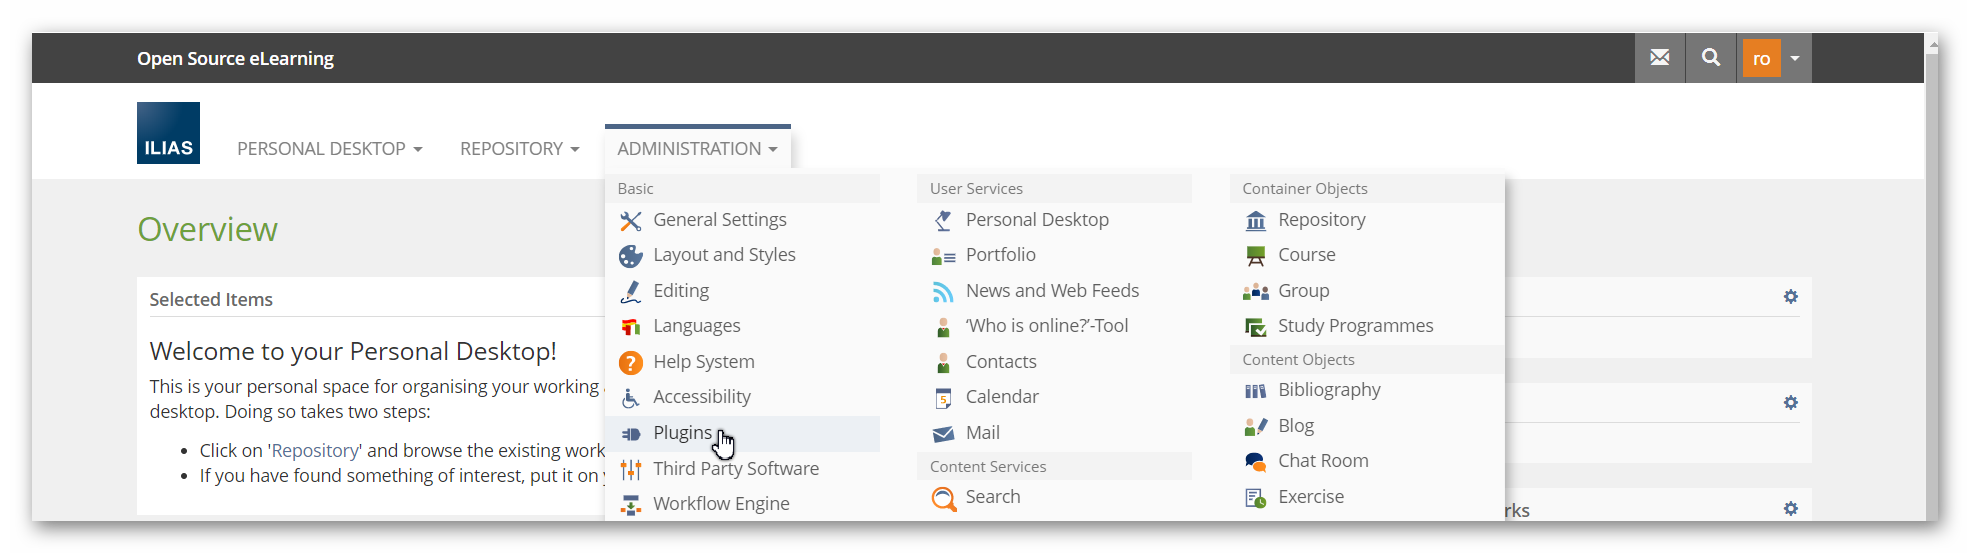
\includegraphics[page=1, width=0.7\paperwidth, trim=4 4 4 4, clip]{fig/Schritt-1-Aktivierung.png} 
                    \caption{Schritt 1 der Aktivierung des \eigenname{assSQLQuestion} Plugins}
                    \label{fig:schritt-1-aktivierung}
                \end{center}
            \end{figure}
    
    \subsubsection{2. Schritt}
    
        Die Installation von \eigenname{assSQLQuestion} erfolgt über die angezeigte \glqq\textit{Install}\grqq\ Auswahlmöglichkeit.
        
            \begin{figure}[H]
                \begin{center}
                    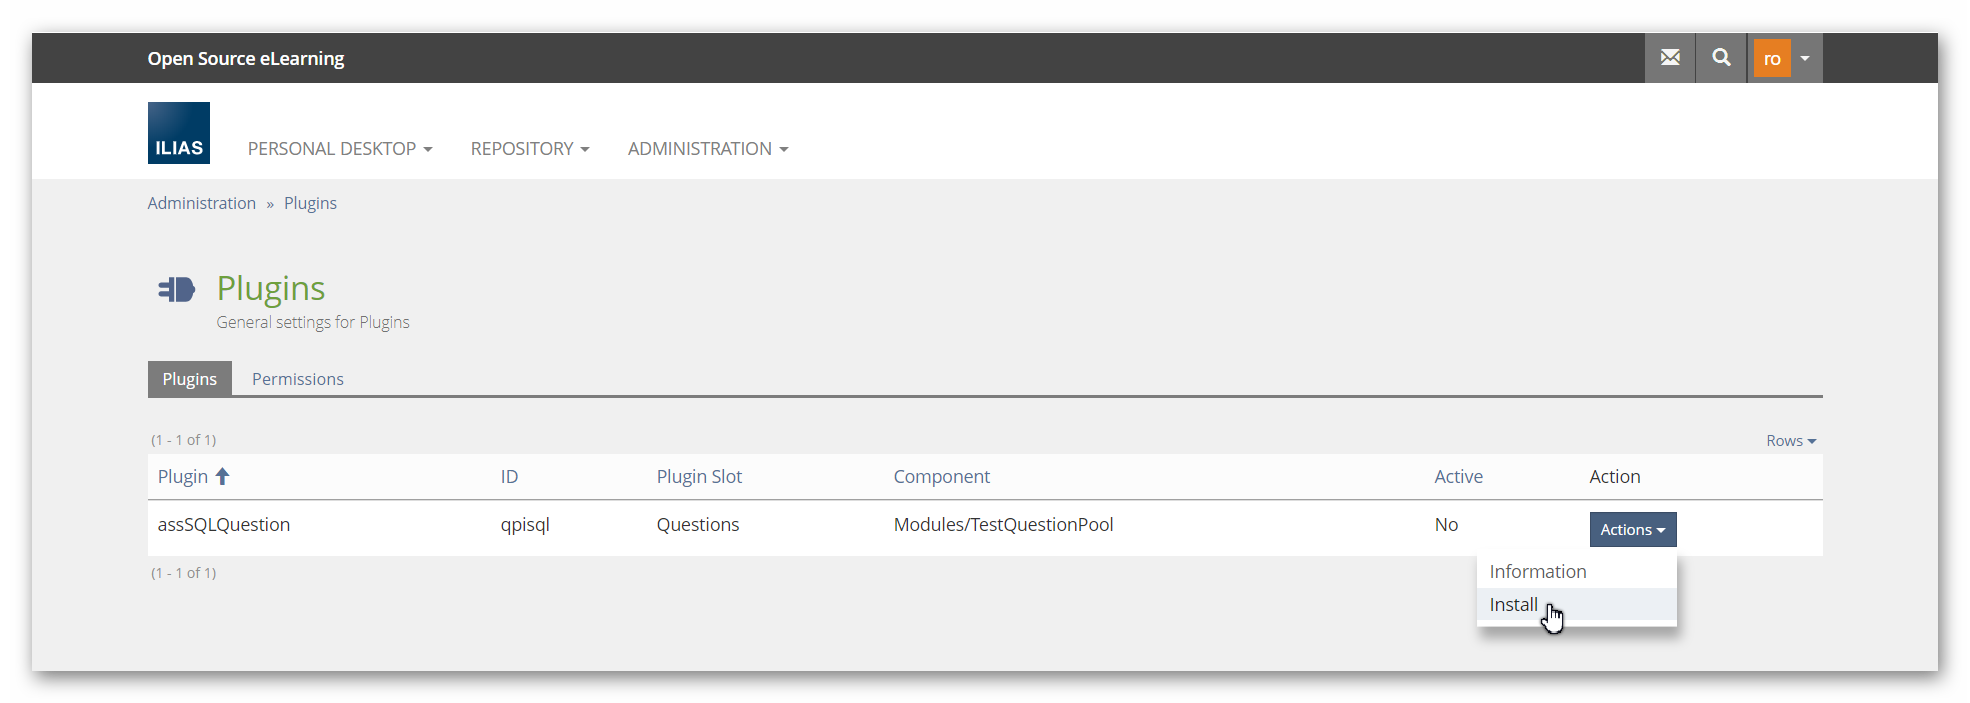
\includegraphics[page=1, width=0.7\paperwidth, trim=4 4 4 4, clip]{fig/Schritt-2-Aktivierung.png} 
                    \caption{Schritt 2 der Aktivierung des \eigenname{assSQLQuestion} Plugins}
                    \label{fig:schritt-2-aktivierung}
                \end{center}
            \end{figure}
    
    \subsubsection{3. Schritt}
    
        Abgeschlossen werden kann die Einrichtung über einen Klick auf die \glqq\textit{Activate}\grqq\ Auswahlmöglichkeit.
        
            \begin{figure}[H]
                \begin{center}
                    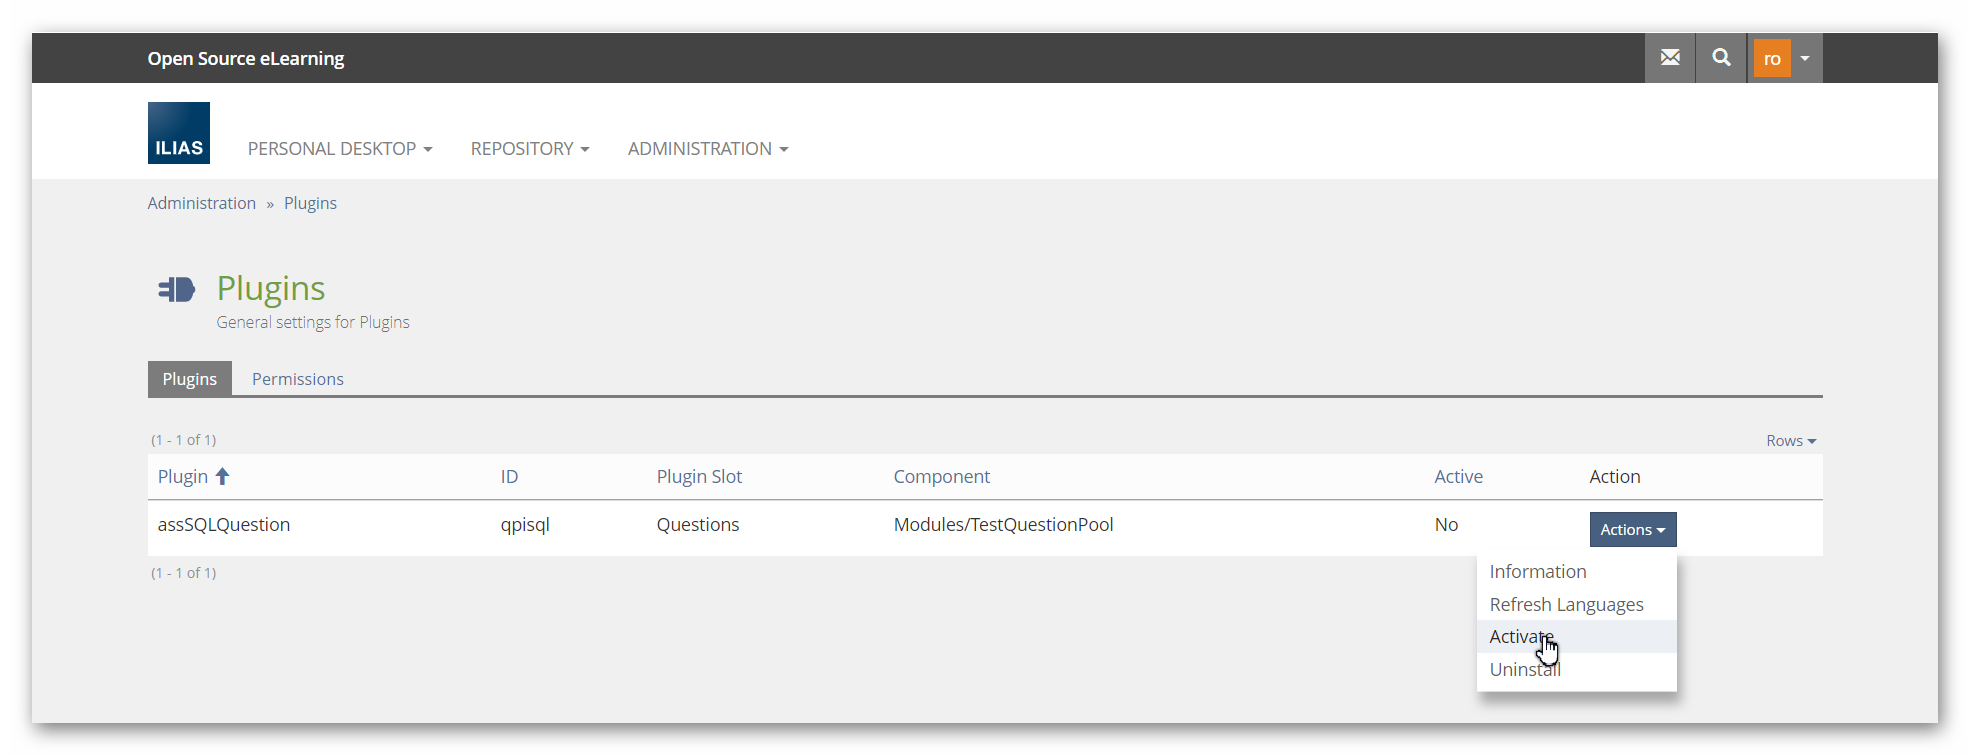
\includegraphics[page=1, width=0.7\paperwidth, trim=4 4 4 4, clip]{fig/Schritt-3-Aktivierung.png} 
                    \caption{Schritt 3 der Aktivierung des \eigenname{assSQLQuestion} Plugins}
                    \label{fig:schritt-3-aktivierung}
                \end{center}
            \end{figure}


\section{Anlegen einer Frage}
\label{sec:anlegen-einer-frage}

Das Anlegen einer allgemeinen Frage in \eigenname{ILIAS} wird grundsätzlich in der User-Dokumentation von \eigenname{ILIAS} (s. \cite{IliasAutorenDokumentation}, Kapitel 14) beschrieben. Bei der \eigenname{assSQLQuestion} gibt es aber einige Besonderheiten, die zu beachten sind. Hier wird abschnittsweise durch diese geführt.

Dabei sei zu erwähnen, dass der Fragetyp, den \eigenname{assSQLQuestion} bereitstellt, bei deutscher Spracheinstellung den Namen \glqq\textit{Interaktive SQL Frage}\grqq\ trägt. Das englische Äquivalent dazu ist in \textbf{Abbildung \ref{fig:create-question}} zu sehen und heißt \glqq\textit{Interactive SQL Question}\grqq .

    \begin{figure}[H]
        \begin{center}
            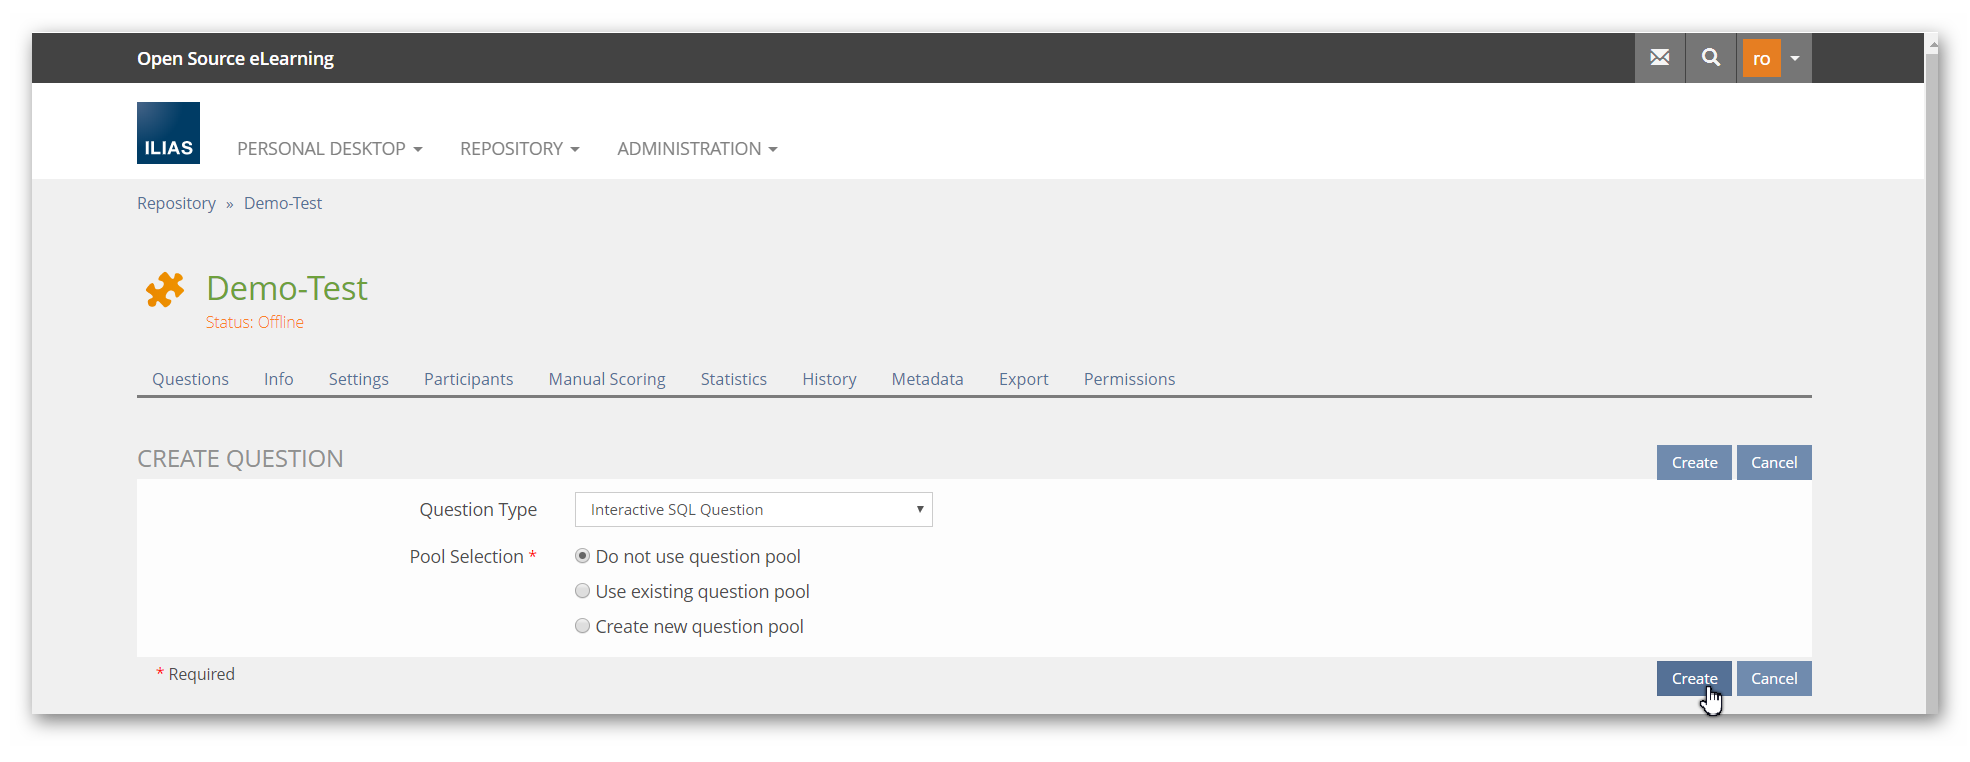
\includegraphics[page=1, width=0.7\paperwidth, trim=4 4 4 4, clip]{fig/Create-Question.png} 
            \caption{Anlegen einer neuen interaktiven SQL Frage}
            \label{fig:create-question}
        \end{center}
    \end{figure}
    
\subsection{Teil 1: Die SQL-Sequenzen}

    Der erste \eigenname{assSQLQuestion} spezifische Teil beim Anlegen einer \glqq\textit{Interaktive SQL Frage}\grqq\ sind die \glqq\textit{SQL-Sequenzen}\grqq . Dabei besteht eine \glqq\textit{Interaktive SQL Frage}\grqq\ aus bis zu drei verschiedenen dieser Sequenzen - genauer Sequenz A, B und C. Bei einer späteren Ausführung werden diese drei Sequenzen gemäß Ihrer alphabetischen Reihenfolge ausgeführt. Die Sequenzen A und C werden vom Fragenersteller vorgegeben und sind für den Teilnehmer nicht zu sehen. Sequenz B soll von dem Teilnehmer später selbst erarbeitet werden. Der Fragenersteller muss dazu eine Musterlösung für diese Sequenz bereitstellen, auf deren Basis später der Teilnehmer bewertet wird. Es ist hier ebenfalls zu erwähnen, dass die automatische Korrektur von \eigenname{assSQLQuestion} nicht die Anfragen an sich bewertet, sondern die letzte sichtbare Ausgabe der SQL-Sequenzen vergleicht.
    
    Des weiteren gehört auch der sogenannte \glqq\textit{Integritätscheck}\grqq\ zum Block der \glqq\textit{SQL-Sequenzen}\grqq . Ist dieser aktiviert, werden Veränderungen an der Datenbank in Sequenz B verhindert, indem die Schlüsselworte \glqq CREATE TABLE\grqq\ , \glqq ALTER TABLE\grqq\ , \glqq DROP TABLE\grqq\ , \glqq INSERT INTO\grqq\ , \glqq UPDATE\grqq\  or \glqq DELETE FROM\grqq\ eine erfolgreiche Ausführung verhindern.
    
    Diese freie Definition wurde bewusst gewählt, um \glqq\textit{Interaktive SQL Frage}\grqq\ von zweierlei Art zu ermöglichen:
    
    \subsubsection{Frage zu einer SELECT-Anfrage}
    
        In diesem Fall nutzt der Fragenersteller Sequenz A um die Datenbank mit Inhalten zu füllen und für eine SQL Anfrage vorzubereiten. Sequenz B ist der Teil der vom Testteilnehmer beantwortet werden muss, der Ersteller füllt dennoch eine beispielhafte Sequenz ein, die als Musterlösung zu werten ist. Sequenz C wird nicht benötigt und bleibt dementsprechend leer. Da bei einer SELECT-Anfrage keine Veränderungen erwünscht sind, sollte auch der Integritätscheck aktiviert werden.
        
        \begin{figure}[H]
            \begin{center}
                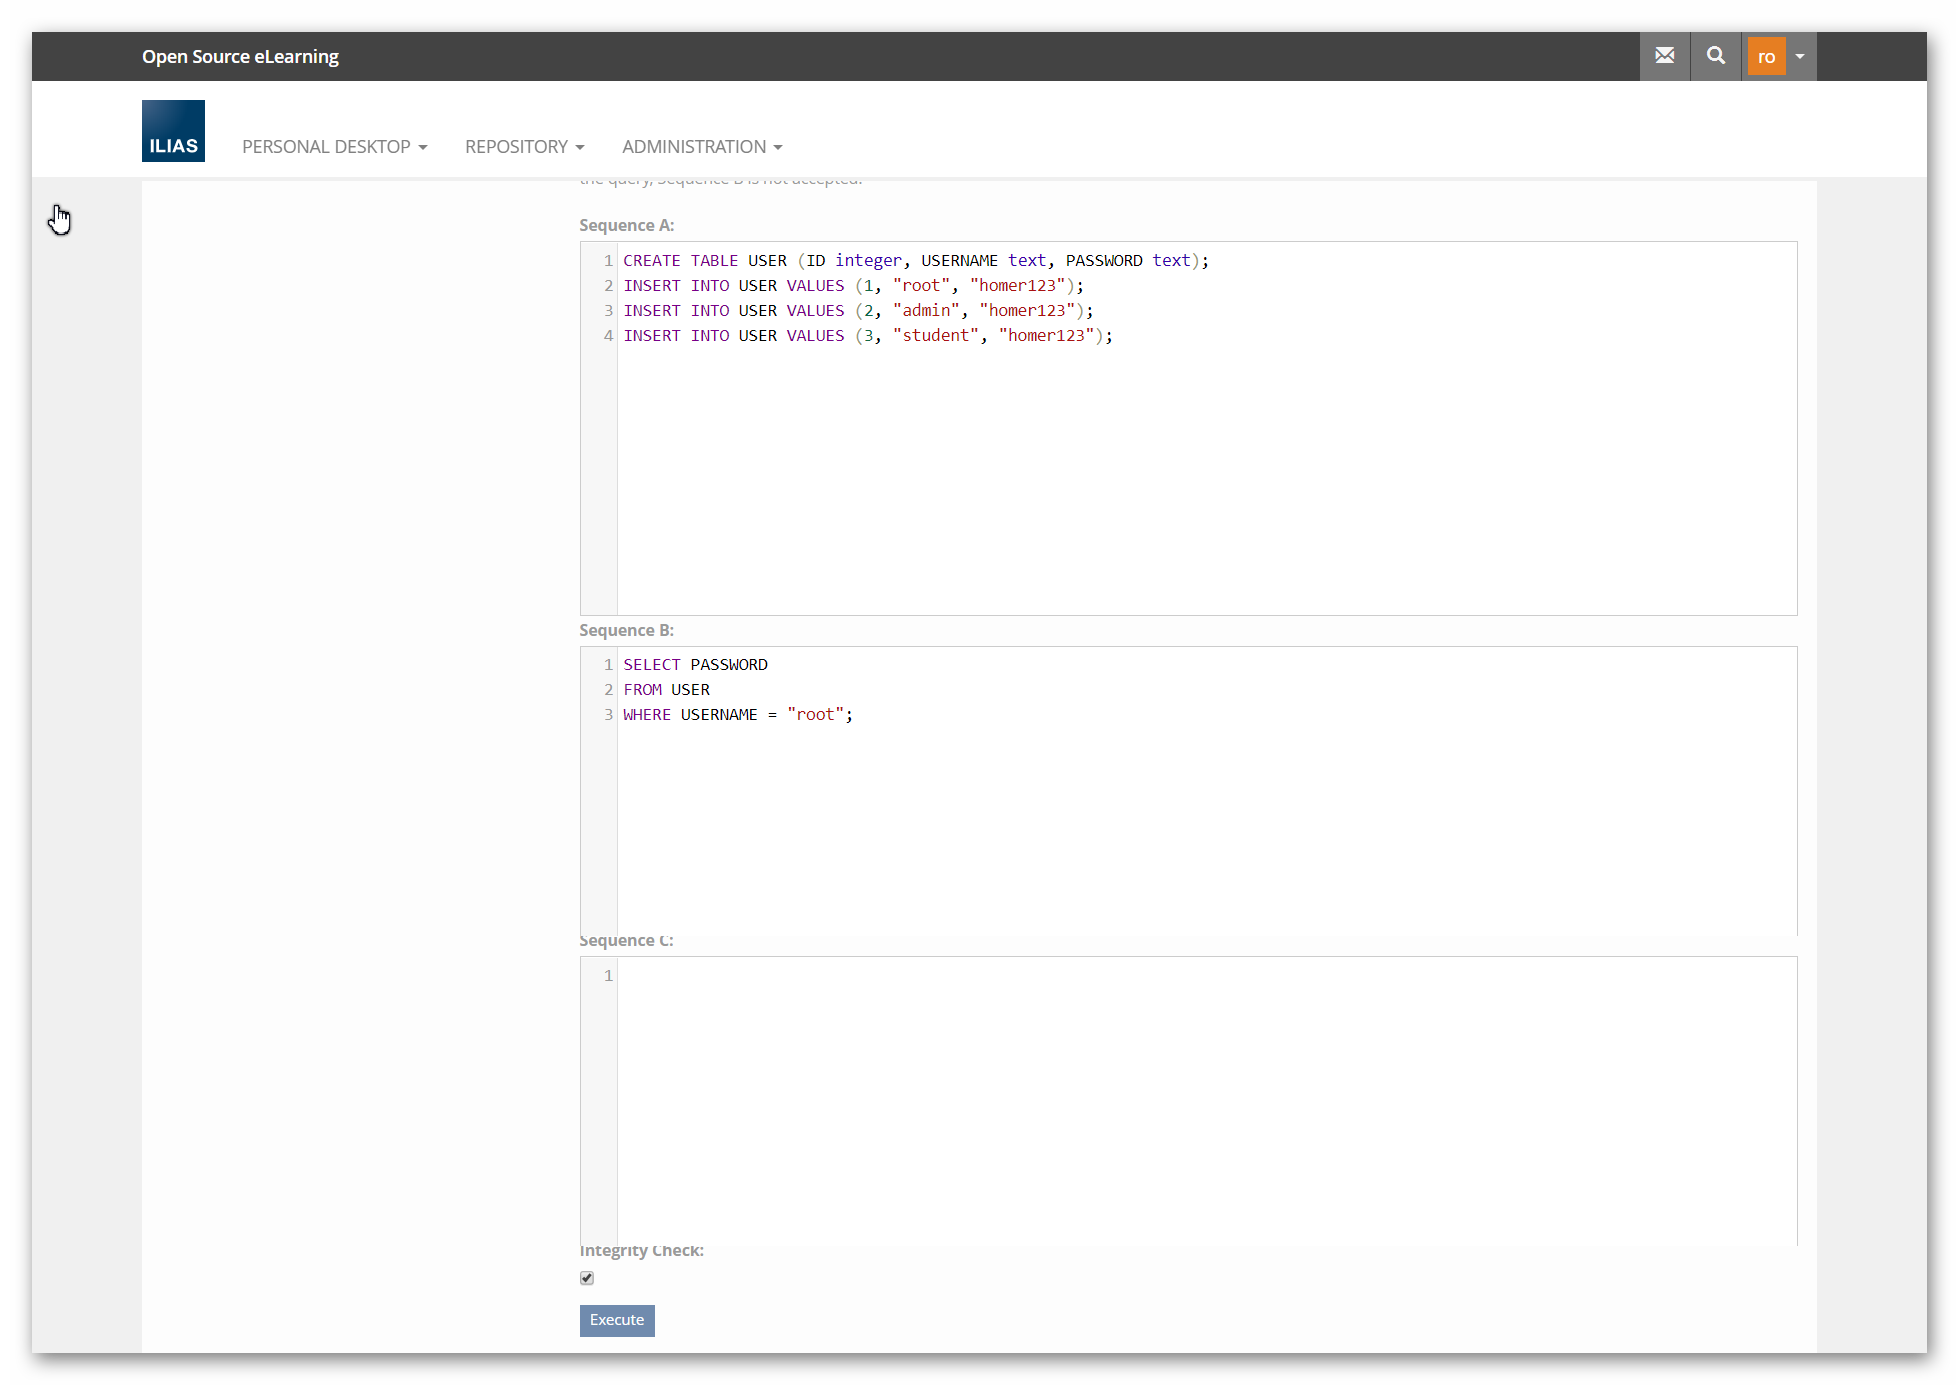
\includegraphics[page=1, width=0.7\paperwidth, trim=4 4 4 4, clip]{fig/Beispiel-SQL-Sequenzen-bei-SELECT-Anfrage.png} 
                \caption{SQL-Sequenzen im Falle einer SELECT Anfrage (Beispiel)}
                \label{fig:beispiel-sql-sequenzen-bei-select-anfrage}
            \end{center}
        \end{figure}
        
    \subsubsection{Frage zu CREATE TABLE, INSERT INTO, DELETE FROM, UPDATE, usw.}
    
        Auch in diesem Fall kann der Frageersteller Sequenz A nutzen um die Datenbank mit Inhalten zu füllen. Dies ist aber von der gewünschten Fragestellung abhängig. Sequenz B ist wieder die Sequenz, die Teilnehmer im Test selbst schreiben müssen. Da die Frage die Fähigkeiten des Teilnehmers prüfen soll CREATE TABLE, INSERT INTO, DELETE FROM, UPDATE und ähnliche Anfragen zu zu beantworten, wird Sequenz B in den meisten Fällen keine SELECT-Anfrage enthalten. Hier ist es wichtig, dass der Testersteller dann in Sequenz C eine Ausgabe erzeugt, da sonst keine Bewertung der Antwort möglich ist. Der Integritätscheck darf dabei nicht aktiviert sein.
        
        \begin{figure}[H]
            \begin{center}
                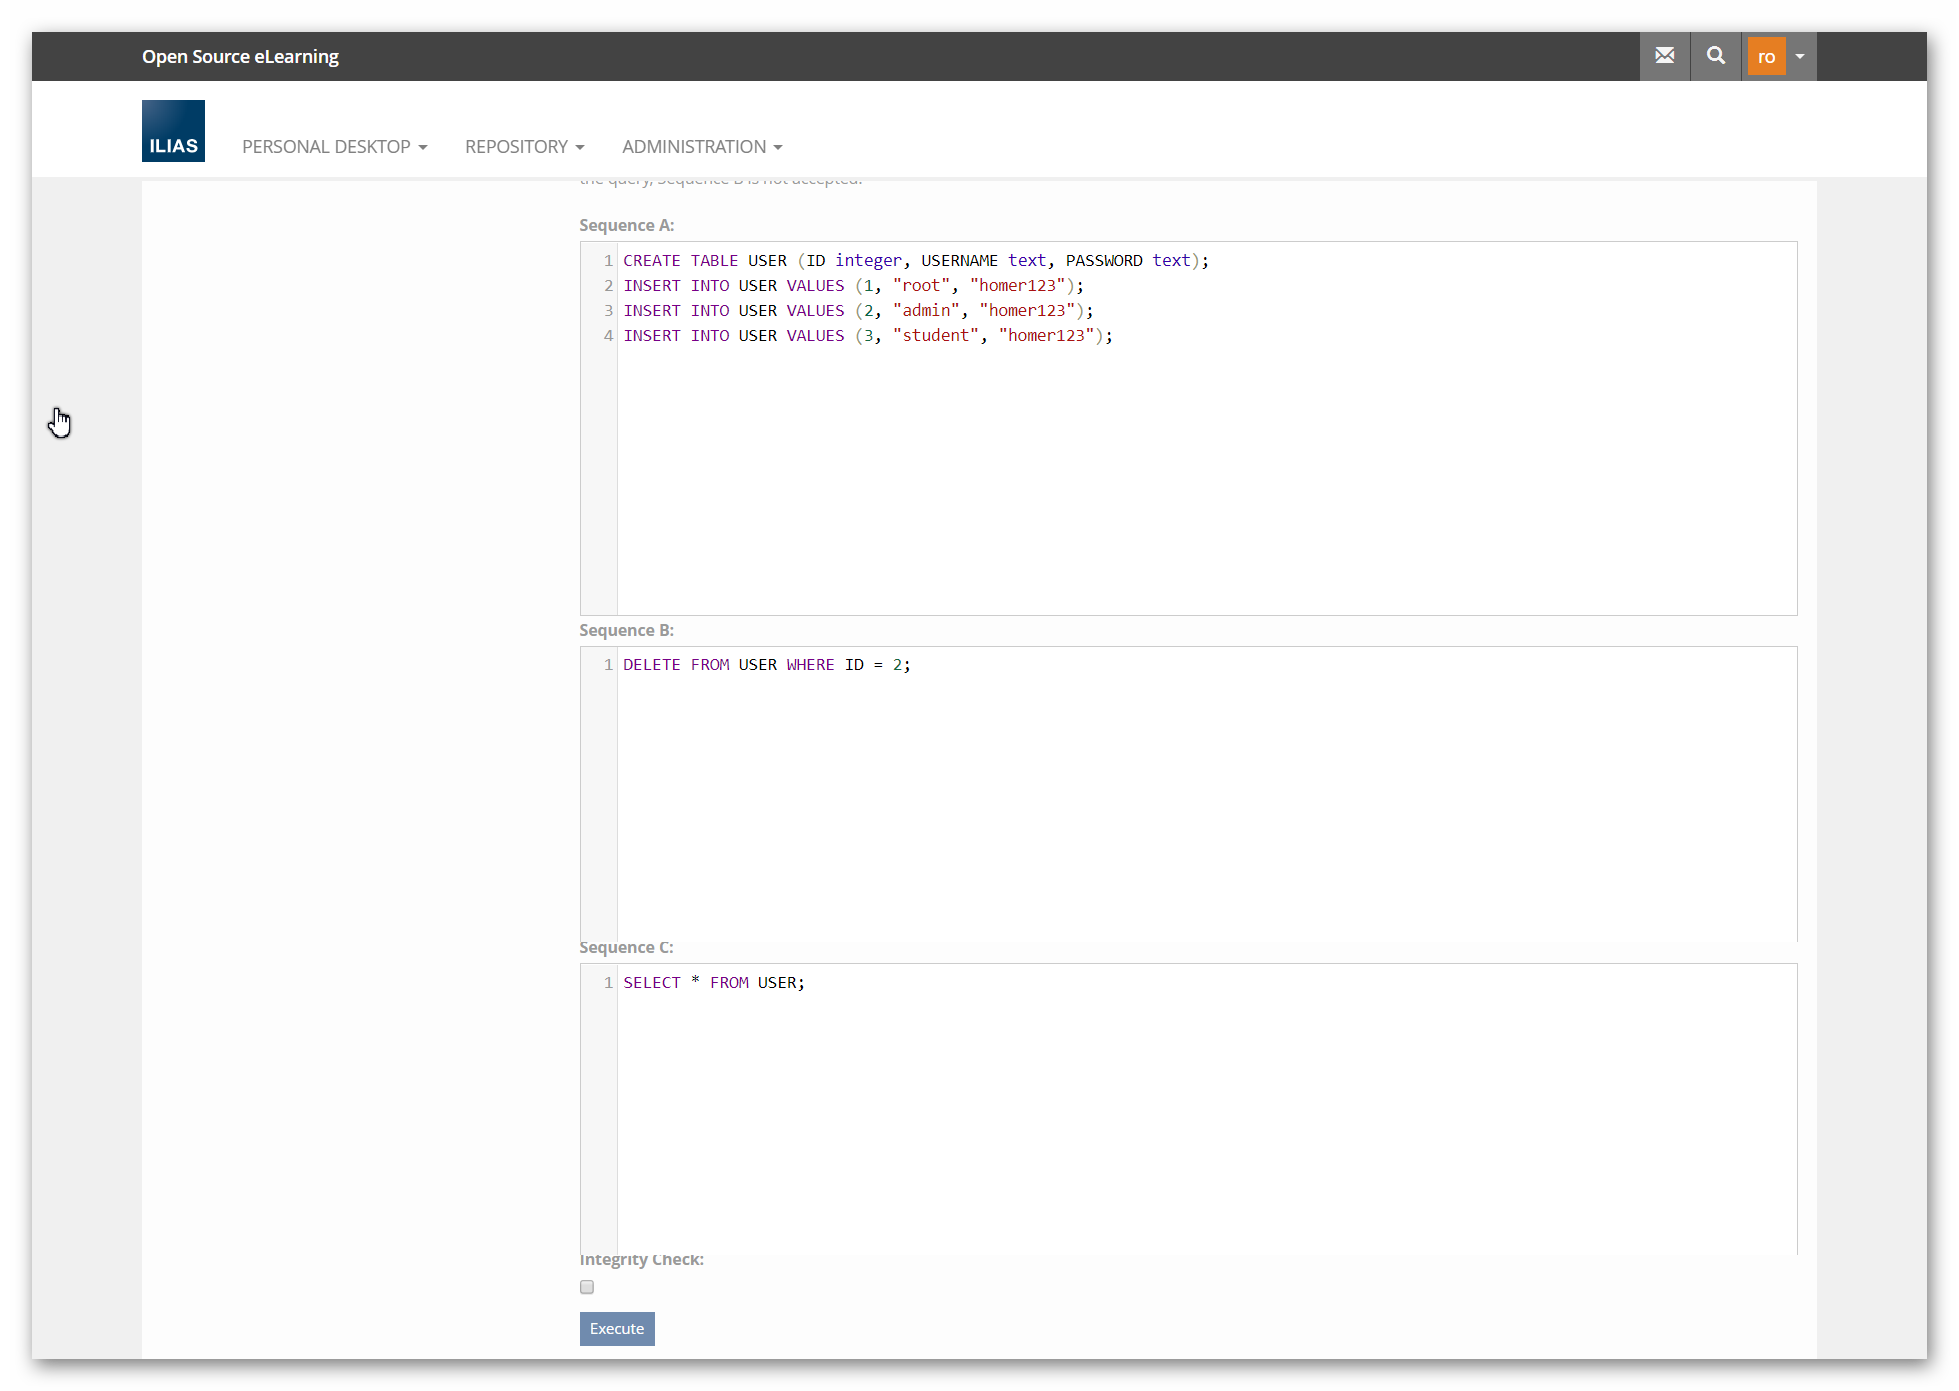
\includegraphics[page=1, width=0.7\paperwidth, trim=4 4 4 4, clip]{fig/Beispiel-SQL-Sequenzen-bei-DELETE-FROM-Anfrage.png} 
                \caption{SQL-Sequenzen im Falle einer DELETE FROM Anfrage (Beispiel)}
                \label{fig:beispiel-sql-sequenzen-bei-delete-from-anfrage}
            \end{center}
        \end{figure}
        
\subsection{Teil 2: Die Ausgabe}
            
        Die Ausgabe wird bei einem Druck auf \glqq\textit{Ausführen}\grqq\ (Englische Spracheeinstellung: \glqq\textit{Execute}\grqq ) automatisch erzeugt. Bei der Erstellung einer Frage ist zu beachten, dass in der Ausgabe keine Fehlermeldung anzeigen werden darf. Außerdem ist es selbstverständlich hilfreich die Ausgabe auf ein erwartetes Ergebnis zu überprüfen.
        
        \begin{figure}[H]
            \begin{center}
                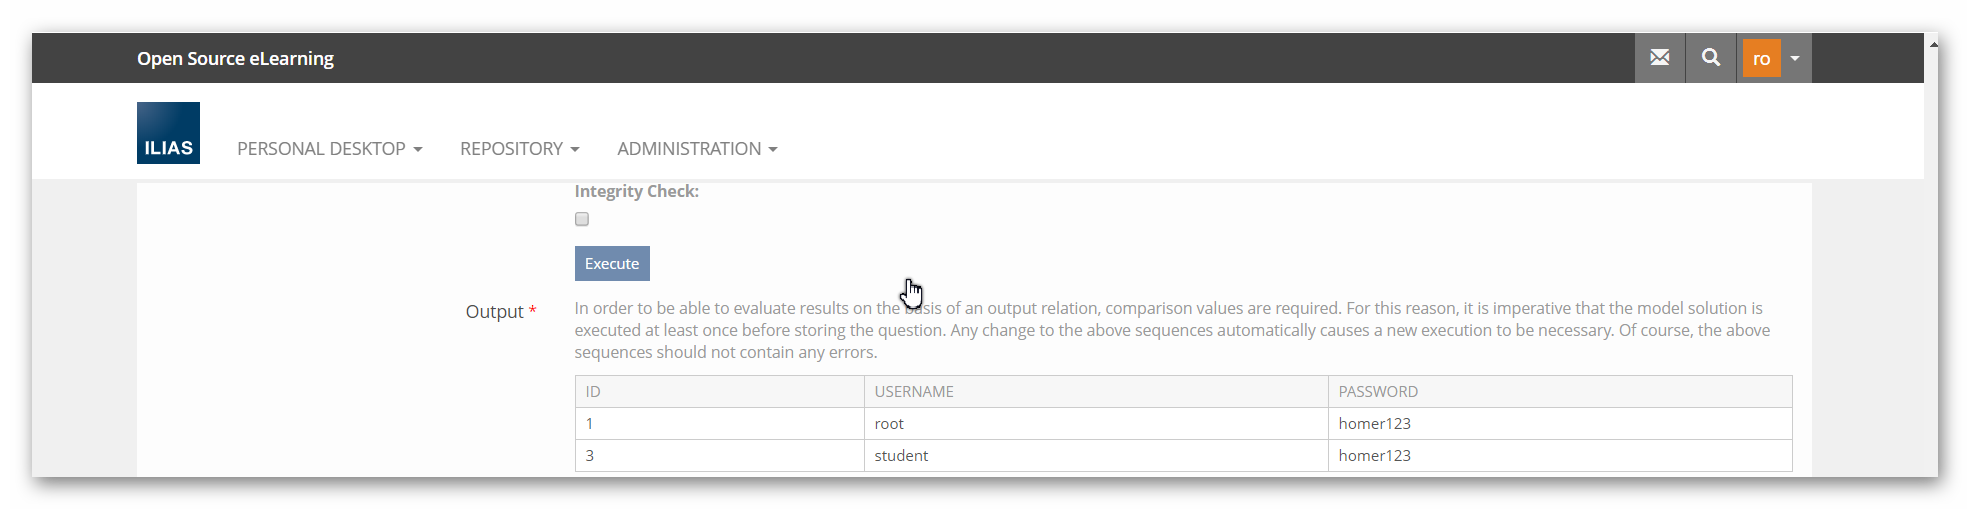
\includegraphics[page=1, width=0.7\paperwidth, trim=4 4 4 4, clip]{fig/Beispiel-Ausgabe-DELETE-FROM.png} 
                \caption{Ausgabe bei SQL-Sequenzen aus \textbf{Abbildung \ref{fig:beispiel-sql-sequenzen-bei-delete-from-anfrage}}}
                \label{fig:beispiel-ausgabe-delete-from-anfrage}
            \end{center}
        \end{figure}
        
\subsection{Teil 3: Die Bepunktung}

        Ein letzter wichtiger Teil, der bei der Erstellung einer Frage zu beachten ist, ist die Bepunktung. Allgemein gesprochen handelt es sich dabei um verschiedene Metriken, die jeweils über die letzte Ausgabe der Musterlösung und die letzte Ausgabe der Antwort des Teilnehmers gelegt werden, um eine Punktzahl für die jeweilige Antwort zu errechnen. Dabei kann der Frageersteller jeder verfügbaren Metrik eine gewisse Punktzahl zuteilen, die ein Teilnehmer maximal in Hinsicht auf diese Metrik erzielen kann. Die Punktzahlen der verschiedenen Metriken addieren sich dann zur Gesamtpunktzahl. Dabei muss die maximal mögliche Gesamtpunktzahl immer positiv sein, um eine Frage erfolgreich anzulegen. Das heißt, dass mindestens für eine verfügbare Metrik eine Maximalpunktzahl größer Null haben muss. 
        
        Zum Release von \eigenname{assSQLQuestion} sind insgesamt drei Metriken verfügbar: \glqq\textit{Anzahl der Tupel}\grqq\ (engl. \glqq\textit{Number of Tuples}\grqq), \glqq\textit{Namen der Attribute}\grqq\ (engl. \glqq\textit{Names of the attributes}\grqq) und \glqq\textit{Funktionale Abhängigkeiten}\grqq\ (engl. \glqq\textit{Functional Dependencies}\grqq). Die Funktionsweise dieser drei Metriken wird im Folgenden erläutert:
        
        \subsubsection{Anzahl der Tupel}
        
            Dies ist die technisch einfachste der drei Metriken. Hierbei werden die Tupel in der Ausgabe gezählt und miteinander verglichen. Hat die Ausgabe des Testteilnehmers identisch viele Tupel wie die Ausgabe der Musterlösung, so bekommt der Teilnehmer die maximale Punktzahl für diese Metrik, in jedem anderen Fall erhält er keine Punkte.
            
            \begin{figure}[H]
                \begin{center} 
                    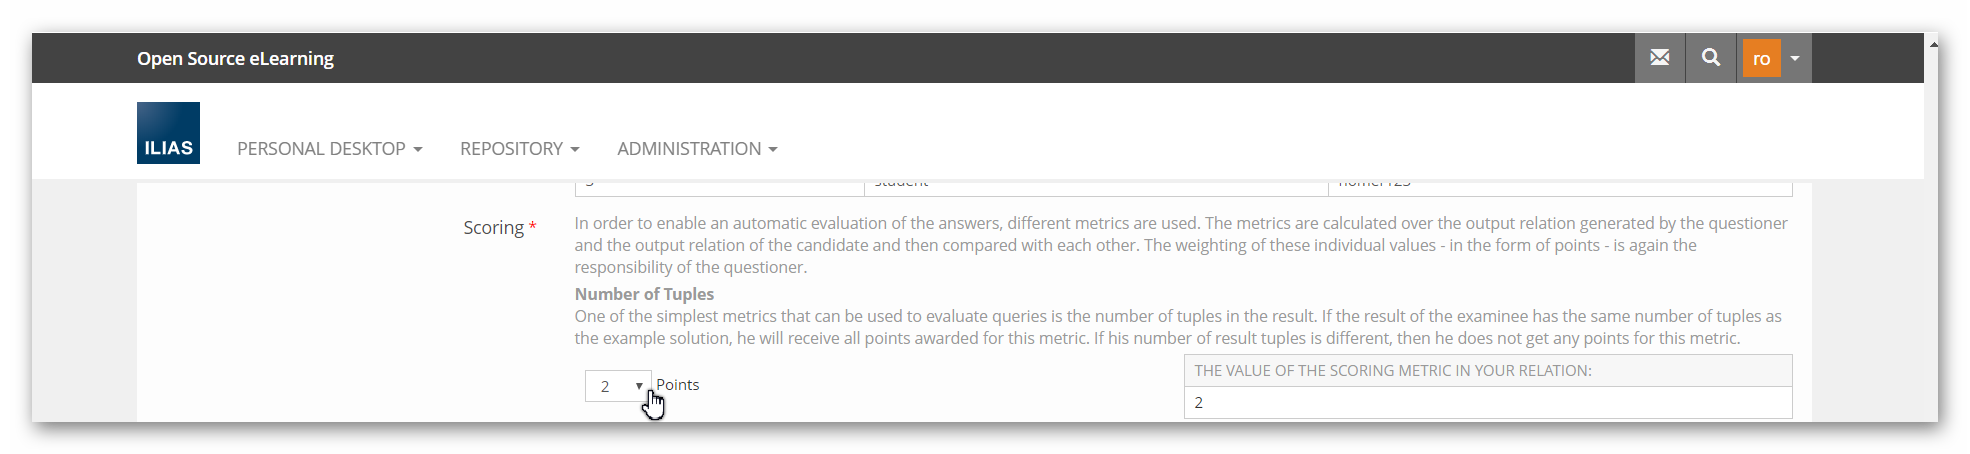
\includegraphics[page=1, width=0.7\paperwidth, trim=4 4 4 4, clip]{fig/Beispiel-Anzahl-der-Tupel-DELETE-FROM.png} 
                    \caption{Anzahl der Tupel zu \textbf{Abbildung \ref{fig:beispiel-sql-sequenzen-bei-delete-from-anfrage}}}
                    \label{fig:beispiel-anzahl-der-tupel-delete-from-anfrage}
                \end{center}
            \end{figure}
            
        \subsubsection{Namen der Attribute}
        
            Diese Metrik vergleicht die Bezeichner der Attribute miteinander. Dabei ist die Ordnung und auch die Groß-/Kleinschreibweise der Bezeichner irrelevant. Berechnet wird die Punktzahl über die Jaccard-Distanz: $ Punkte = MaxPunkte * (1 - JaccardDistanz) $. Es wird dabei nicht gerundet, wodurch auch im Gesamtergebnis mit ungerundeten Punktzahlen zu rechnen ist.
            
            Wenn Prüfungsteilnehmer ihre Bezeichner frei wählen dürfen, sollte die maximale Punktzahl bei dieser Metrik logischerweise Null entsprechen.
            
            \begin{figure}[H]
                \begin{center}
                    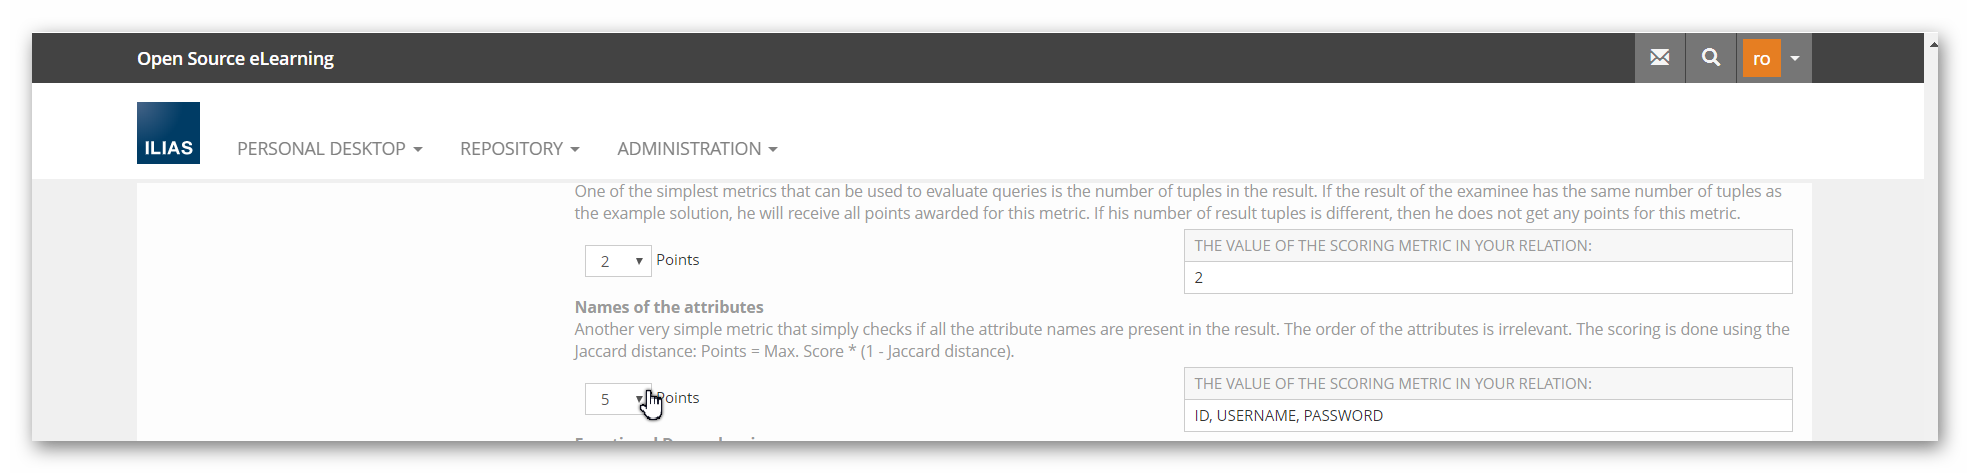
\includegraphics[page=1, width=0.7\paperwidth, trim=4 4 4 4, clip]{fig/Beispiel-Namen-der-Attribute-DELETE-FROM.png} 
                    \caption{Namen der Attribute zu \textbf{Abbildung \ref{fig:beispiel-sql-sequenzen-bei-delete-from-anfrage}}}
                    \label{fig:beispiel-namen-der-attribute-delete-from-anfrage}
                \end{center}
            \end{figure}
            
        \subsubsection{Funktionale Abhängigkeiten}
        
            Die Metrik zu den funktionalen Abhängigkeiten ist die komplexeste der drei Metriken. Dabei werden zu den Ausgaben zunächst alle enthaltenen funktionalen Abhängigkeiten bestimmt, wobei in einem zweiten Schritt alle \glqq nicht minimalen\grqq\ Abhängigkeiten entfernt werden. Genauer heißt das, dass funktionale Abhängigkeiten bei denen bereits ein Bestandteil der Determinante die gleichen Attribute bestimmt, nicht für die Metrik verwendet werden. 
            
            Der übrige Pool von funktionalen Abhängigkeiten innerhalb der Ausgabe der Musterlösung, wird dann der Menge aus funktionalen Abhängigkeiten aus dem Ergebnis des Teilnehmers gegenüber gestellt. Hier wird, wie bei der Metrik zu den Namen der Attribute, eine ordnungsignorierende Jaccard-Distanz verwendet. Auch die Groß-/Kleinschreibung wird ignoriert und die Reihenfolge der Attribute in den funktionalen Abhängigkeiten werden Reihenfolge insensitiv behandelt. Die berechnende Formel ist auch hier wieder: $ Punkte = MaxPunkte * (1 - JaccardDistanz) $.
            
            \begin{figure}[H]
                \begin{center}
                    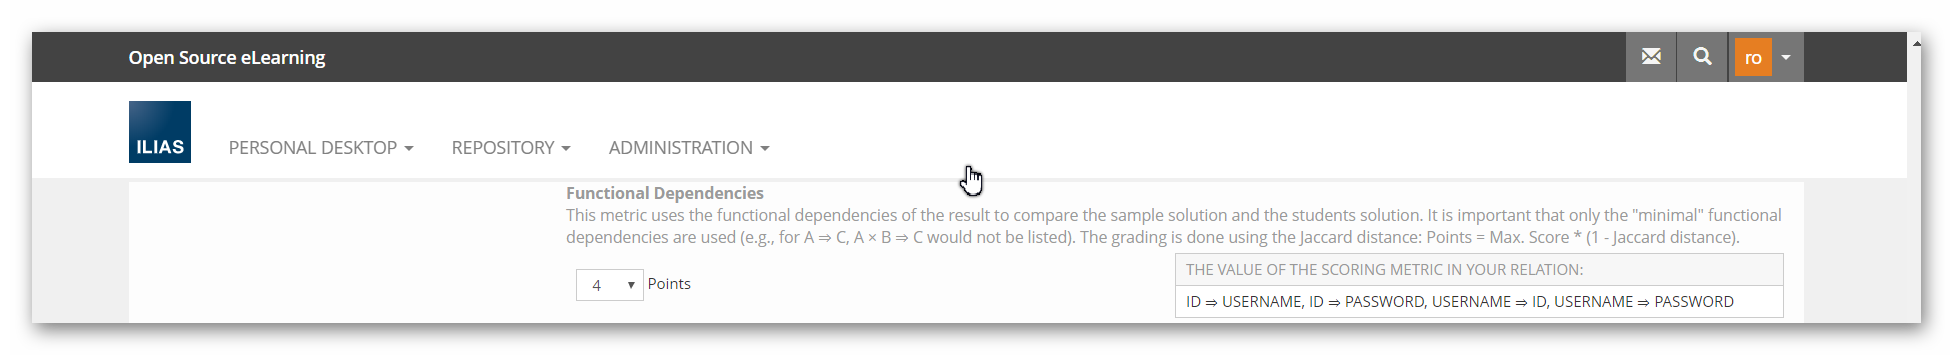
\includegraphics[page=1, width=0.7\paperwidth, trim=4 4 4 4, clip]{fig/Beispiel-Funktionale-Abhaengigkeiten-DELETE-FROM.png} 
                    \caption{Funktionale Abhängigkeiten zu \textbf{Abbildung \ref{fig:beispiel-sql-sequenzen-bei-delete-from-anfrage}}}
                    \label{fig:beispiel-funktionale-abhaengigkeiten-delete-from-anfrage}
                \end{center}
            \end{figure}

\chapter{Zusammenfassung}
	TODO Zusammenfassung



\backmatter
\printbibliography
%\bibliographystyle{unsrt}
%\bibliography{bib/literatur}
%\nocite{*}

\end{document}
